\chapter{UNIX}

\lstset{language=bash}
Viele der Grundprinzipien von UNIX sind in heutigen Betriebssystemen noch vorhanden und mit einigen dieser Betriebssysteme wirst du im laufe eures Studiums noch zu tun haben.

\section{Verzeichnisstruktur}
In Unix wird alles, egal ob es sich um eine Netzwerkschnittstelle, die Festplatte oder eine Musikdatei handelt als Datei repräsentiert. Alle diese Dateien lassen sich im sogenannten „Verzeichnissbaum“ des Betriebssystems finden. Das wohl wichtigste Verzeichnis in UNIX ist \lstinline$/$ – das Wurzelverzeichnis. In diesem Verzeichnis liegen alle anderen Verzeichnisse.

An dieser Stelle lernst du die ersten beiden Kommandos für das Terminal kennen: \lstinline$ls$ und \lstinline$cd$.
Sie sind die wichtigsten Kommandos für die Navigation durch den Verzeichnissbaum von Unix. \lstinline$cd$ steht für „change directory“ und lässt uns das Verzeichnis wechseln. Gibt man also \lstinline$cd /$ ins Terminal ein, so wechselt man ins Wurzelverzeichnis. \lstinline$ls$ steht für „list search“, es liefert eine Auflistung der Dateien im aktuellen Ordner.
Da in Unix alles eine Datei ist, sieht man auch die Unterverzeichnisse des aktuellen Verzeichnisses.
Die Verzeichnisse im Wurzelverzeichnis sind bei den meisten Betriebssystemen (fast) gleich und jedes dieser Verzeichnisse erfüllt die selbe Bedeutung.

\begin{table}
\centering
\begin{tabular}{l|l}
Verzeichnis & Bedeutung \\ \hline
\lstinline$/$ & das Wurzelverzeichnis \\
\lstinline$/bin$ & Ausführbare Programme, z.B. die Shell /bin/sh \\
\lstinline$/boot$ & der Betriebssystemkern und was zum hochfahren benötigt wird \\
\lstinline$/dev$ & „Devices“ zum Beispiel Festplatten, USB-Geräte, der Zufallszahlengenerator ...\\
\lstinline$/etc$ & Konfigurationsdateien für das Betriebssystem \\
\lstinline$/home$ & Das Elternverzeichnis aller Nutzerverzeichnisse \\
\lstinline$/lib$ & Bibliotheken für andere Programme \\
\lstinline$/opt$ & manuell installierte Programme \\
\lstinline$/proc$ & Systemressourcen \\
\lstinline$/root$ & Das Heimatverzeichnis des „root“-Nutzers \\
\lstinline$/sbin$ & das „bin“ für Programme die nur root ausführen darf \\
\lstinline$/tmp$ & Temporäre Dateien \\
\lstinline$/usr$ & „unix system resources“ Dateien die für alle Nutzer relevant sind \\
\lstinline$/var$ & Variabler Inhalt, in \lstinline$/var/log$ verstecken sich diverse Log-Files
\end{tabular}
\label{UNIX-Verzeichnisse}
\end{table}

Außerdem gibt es noch Kurzschreibweisen für bestimmte Verzeichnisse. \lstinline$.$ beszeichnet das aktuelle Verzeichnis, \lstinline$..$ das Elternverzeichnis und \lstinline$~$ das eigene Homeverzeichnis.
Dateien und Verzeichnisse die mit \lstinline$.$ beginnen sind versteckt. Man kann sie anzeigen, wenn man \lstinline$ls$ mit dem Parameter \lstinline$-a$ benutzt.

\section{Arbeiten im Textmodus}
Unix stammt aus Zeiten, in denen man einen Rechner mit mehreren „Terminals“ bedient hat. 
Ist man an so einem Terminal angemeldet, sieht man erstmal die Ausgabe des sog. „Command Line Interpreters“ – \lstinline$/bin/sh$.
Dieses Programm ist im wesentlichen dafür zuständig, andere Programme aufzurufen. Hinter dem Kommando ls versteckt sich zum Beispiel ein Aufruf des Programms \lstinline$/bin/ls$. Außerdem gibt es noch einige zusätzliche Kommandos, wie \lstinline$help$ die direkt zum Command Line Interpreter gehören. 

Das vermutlich wichtigste Kommando in Unix ist \lstinline$man$. Mit \lstinline$man$ lassen sich die sogenannten Manpages zu einem Programm anzeigen. In der Manpage stehen alle wichtigen Informationen, die man zu einem Programm braucht.
\lstinline$man man$ gibt zum Beispiel eine Hilfeseite zur Benutzung dieser Manpages aus.

\begin{table}
\centering
\begin{tabular}{l|l}
Befehl & Bedeutung \\ \hline
\lstinline$cat$ & gibt den Inhalt einer Datei aus \\
\lstinline$cd$ & Verzeichnis wechseln \\
\lstinline$cp$ & kopiert eine Datei \\
\lstinline$date$ & zeigt das aktuelle Datum und die Uhrzeit an \\
\lstinline$echo$ & gibt die Eingabe zurück \\
\lstinline$exit$ & aktuelle Terminalsession beenden \\
\lstinline$gedit$ & ruft einen Texteditor auf \\
\lstinline$grep$ & Durchsuchen einer Datei \\
\lstinline$java$ & ein Javaprogramm ausführen \\
\lstinline$javac$ & Javaquellcode in Bytecode übersetzen \\
\lstinline$ls$ & zeigt den Inhalt des aktuellen Verzeichnisses \\
\lstinline$man$ & zeigt eine Hilfeseite an \\
\lstinline$mkdir$ & legt ein Verzeichnis an \\
\lstinline$mv$ & verschiebt eine Datei \\
\lstinline$passwd$ & eigenes Passwort ändern \\
\lstinline$pwd$ & Zeigt das Verzeichnis mit komplettem Pfad an \\
\lstinline$rm$ & Datei löschen \\
\lstinline$ssh$ & eine Shell auf einem anderen Rechner öffnen \\
\lstinline$tar$ & Dateiarchive packen und entpacken \\
\lstinline$unzip$ & zip-Archive öffnen \\
\lstinline$wget$ & herunterladen einer Datei \\
\lstinline$yes$ & wiederholt die Eingabe
\end{tabular}
\label{Befehle}
\caption{Wichtige Befehle}
\end{table}

\subsection{Befehlssyntax}
Um einen Befehl richtig ausführen zu können benötigt dieser eine bestimmte Form. Ein typischer Unixbefehl könnte so aussehen:
\lstinline$ls -lBh ~/$. ls ist der ausgeführte Befehl, \lstinline$-l$, \lstinline$-B$ und \lstinline$-h$ sind Parameter für das Programm \lstinline$ls$ und \lstinline$~/$ der Pfad zum Verzeichnis, dessen Dateien \lstinline$ls$ auflisten soll. \lstinline$~$ ist eine abgekürzte Schreibweise für das eigene home-Verzeichnis.
Genau so werden die Parameter und der richtige Aufruf von ls auch in der Manpage beschrieben. Mehrere Parameter können oftmals auch zusammengefasst werden, so dass \lstinline$ls -l -a ..$ die selbe Bedeutung hat wie \lstinline$ls -la ..$

\subsection{Befehle verknüpfen}
In Unix können auch mehrere Befehle verknüpft werden. Dazu gibt es mehrere nützliche Operatoren.
\begin{itemize}
\item \lstinline$command &$ führt das Kommando im Hintergrund aus
\item Mit \lstinline$command1 && command2$ kann man mehrere Kommandos hintereinander ausführen z.B. \lstinline$mkdir foo && ls -l && cd foo/$
\item Mit \lstinline$command1 | command2$ kann man die Ausgabe von Kommando1 als Eingabe in Kommando2 verwenden  z.B. \lstinline$ls -l | grep foo$
\end{itemize}

Man kann mit diesen Verknüpfungen aber auch sehr viel Schabernack treiben, man sollte davon nicht mehr benutzen als man benötigt, da man so unnötige Fehler vermeiden kann.

Auch diese Operatoren sind oft nützlich:
\begin{itemize}
\item \lstinline$command > file$ schreibt die Ausgabe der Befehls in die angegebene Datei
\item \lstinline$command >> file$ hängt die Ausgabe hinten an die Datei an
\end{itemize}


\subsection{Vom Textmodus zum Graphikmodus und wieder zurück}
\begin{figure}
	\centering
	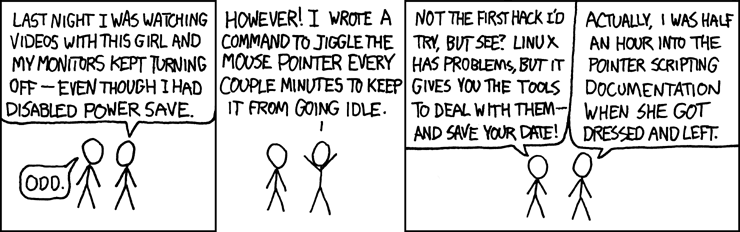
\includegraphics[width=\textwidth]{images/command_line_fu.png}
	\caption{\href{http://xkcd.com/196}{xkcd.com/196}}
\end{figure}
Wie man zum Beispiel in den Rechnerpools der Fakultät sieht, besitzen moderne Unixoide Betriebssysteme nicht mehr ausschließlich den Textmodus. Man kann auch wie gewohnt in Fenstern bunte Bildchen anschauen.

Im Gegensatz zu Windows, kann man hier allerdings Programme nicht wirklich von der Shell losgelöst starten, die Ein- und Ausgaben sind nur für den User nicht mehr sichtbar. 
Besonders deutlich wird wenn man zum Beispiel \lstinline$firefox$ über ein Terminal startet – ob Webbrowser, Spiel oder Programmierumgebung – jedes Programm hängt an der Shell.

Mit dem Befehl \lstinline$ssh$ kann man auch eine Shell auf einem anderen Unix-Rechner öffnen und sich Beispielsweise von Zuhause im Rechnerpool der FIN einloggen und dort arbeiten – sogar mit Programmen die man lokal gar nicht installiert hat. 
Mit \lstinline$ssh -x$ kann man auch Graphikmodus-Programme benutzen.
Im Gegensatz zum Remotedesktop werden hier allerdings wesentlich weniger Daten übertragen und der Computer bleibt (einigermaßen) schnell.

\section {Aufgaben}

\begin{itemize}
\item lade dir mit \lstinline$wget ...$ das Dateiarchiv für die erste Aufgabe herunter, entpacke es mit \lstinline$tar -xf$.
\item sieh nach wie spät es ist mit \lstinline$date$ und rufe mit \lstinline$man date$ die Manpage zu \lstinline$date$ auf
\item lege in Europa einen Ordner 'Großbritanien' an und verschiebe 'york' hinein
\item finde Atlantis und lösche es
\item lege einen weiteren Ordner mit Städten für Australien an, lösche den Ordner wieder
\item trage die Einwohnerzahl von Magdeburg in der Datei europa/deutschland/magdeburg ein
\item gib den Inhalt der Datei europa/deutschland/magdeburg mit \lstinline$cat$ aus
\item schau dir die Dateien in deinem Homeverzeichnis an
\item öffne eine ssh-Verbindung zu \lstinline$trex.cs.uni-magdeburg.de$ (anmelden kann man sich dort mit seinem FIN-Account.
\end{itemize}
